\documentclass[main.tex]{subfiles}

\begin{document}
	
	\newpage
	\listoffigures{}
	\newpage
	
\section{Постановка задачи}
	Есть установка — токамак, маленький термоядерный реактор. В нем проводятся эксперименты — короткие разряды. \cite{tok} У каждого разряда токамака — отдельный файл типа «.sht».
	У разрядов существуют шумы и выбросы. Они «плохие» и мешают работе данными.
	Имеется алгоритм - реализованный Гареевой М., способный выделять области развития процесса, в которых предполагается наличие полезных сигналов (процессов).\\
	Надо проверить насколько устойчиво работает алгоритм.
	
\section{Теория}
	\subsection{Введение}
		У разрядов токамака существуют артефакты – это отдельные выбросы и шумы.
	\subsection{Шумы}
		Шумы – это горизонтальные участки разряда. Они означают, что аппаратура стала «деревянной», на время потеряла чувствительность. Такие участки могут быть только до и после полезного сигнала, на нем они быть не могут.
	\subsection{Выбросы}
		Выбросы — это экстремальные значения во входных данных, которые находятся далеко за пределами других наблюдений. Их очень легко увидеть: если точка сильно «улетела» вверх или вниз, то она является выбросом. Это помехи, поскольку реальные сигналы меняются относительно медленно.
		
\section{Реализация}
	Лабораторная работа выполнена с помощью языка программирования Python. Исходный код лабораторных работ приведён в Githab.
	
	Работа по удалению шумов и сглаживанию выбросов начинается в функции:\\
	\textbf{def process(timestamp, signal, step=100)}, у которой следующие входные параметры:
	\begin{enumerate}
		\item signal – весь сигнал;
		\item step – размер шага (окно), с которым мы идем по сигналу.
	\end{enumerate}

	Сначала нам нужно удалить шумы. Поэтому с помощью построенной гистограммы \cite{hist} мы находим границы 2-ух самых больших ее столбцов.\\ Далее вызывается функция \textbf{getusefulsignalboundaries(signal, (edges[idx1], edges[idx1 + 1]), step)}, новые входные параметры которой отвечают за границы самого высокого столбика гистограммы и следующего за ним. По названию можно понять, что после отработки этой функции мы получим левую и правую границы полезного сигнала, то есть избавимся от шумов.\\
	Что происходит в этой функции? Мы идем по сигналу слева направо, а затем справа налево каким-то окном размера step. То есть мы берем часть сигнала размера step и смотрим, какие значения этой части находятся внутри границ нашего самого большого столбика гистограммы. Если процентное соотношение количества значений больше параметра \underline{threshold}, то мы нашли участок шума.\\
	
	Проверим насколько устойчив алгоритм к изменениям параметра \underline{threshold}\\
	Будем его менять начиная с $0.01$ до $0.97$ с шагом $0.2$ и отдельно рассмотрим $0.98$ и $0.99$ - пороговые значения должны быть интересны.\\
	
\section{Результаты}
	Для следующих рисунков: Сигнал 20 и его гистограмма до (два рисунка сверху) и после обработки (рисунки снизу), файл sch38515\\
	\begin{figure}[H]
		\center{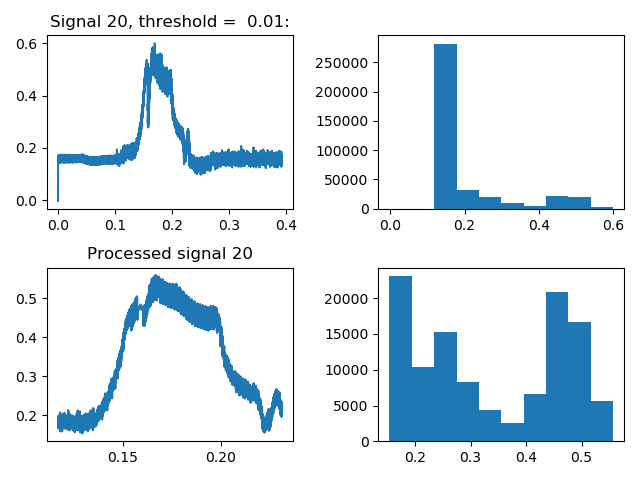
\includegraphics{threshold = 0.01 Num = 0 ShotNo= 38515 Signal= 20}}
		\caption{Параметр threshold = 0.01}
		\label{fig:threshold = 0.01}
	\end{figure}

	\begin{figure}[H]
		\center{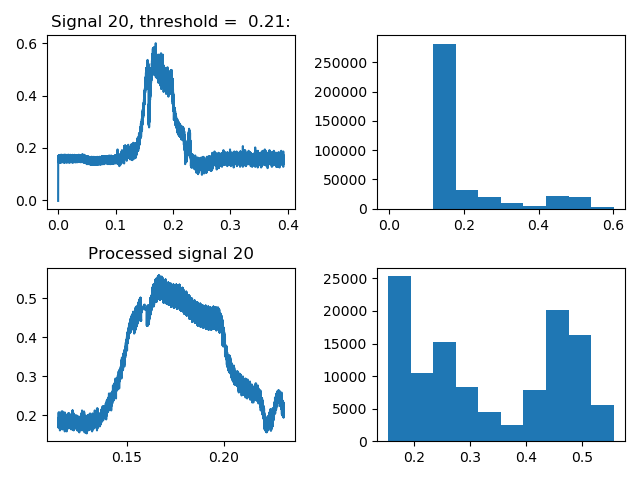
\includegraphics{threshold = 0.21 Num = 2 ShotNo= 38515 Signal= 20}}
		\caption{Параметр threshold = 0.21}
		\label{fig:threshold = 0.21}
	\end{figure}

	\begin{figure}[H]
		\center{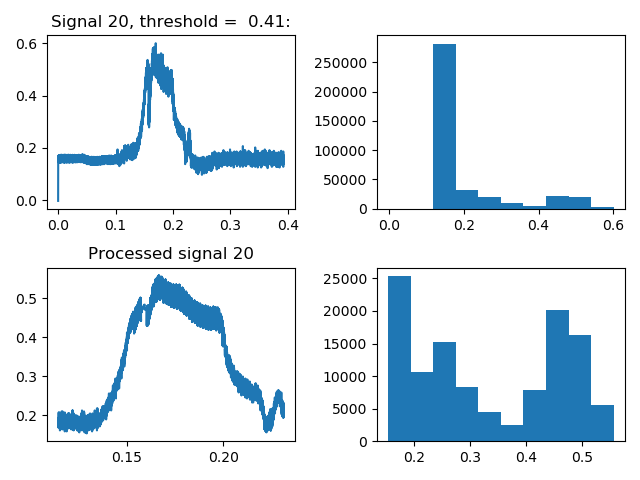
\includegraphics{threshold = 0.41 Num = 4 ShotNo= 38515 Signal= 20}}
		\caption{Параметр threshold = 0.41}
		\label{fig:threshold = 0.41}
	\end{figure}

	\begin{figure}[H]
		\center{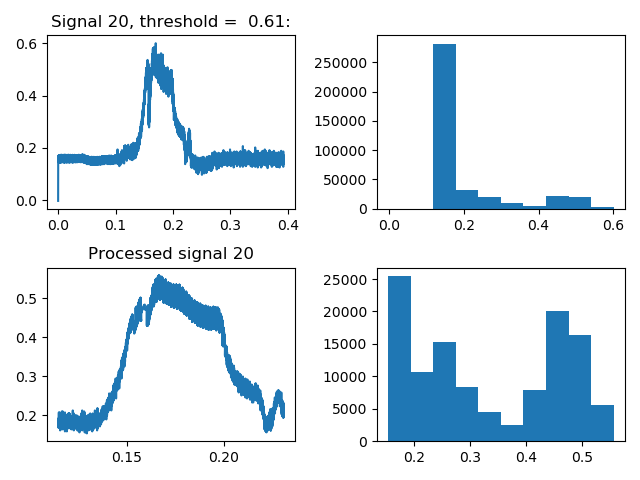
\includegraphics{threshold = 0.61 Num = 6 ShotNo= 38515 Signal= 20}}
		\caption{Параметр threshold = 0.61}
		\label{fig:threshold = 0.61}
	\end{figure}

	\begin{figure}[H]
		\center{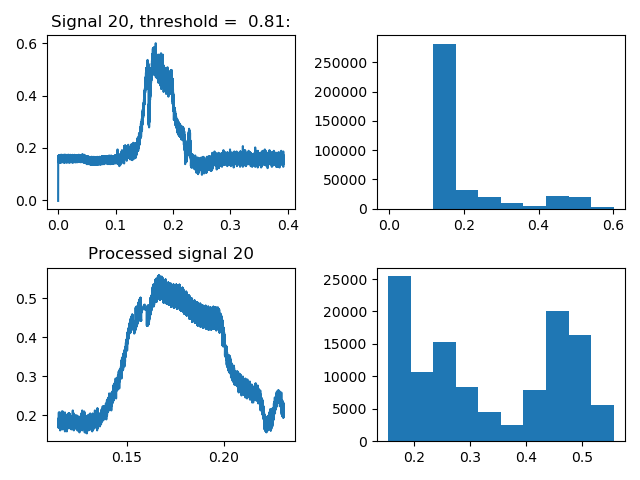
\includegraphics{threshold = 0.81 Num = 8 ShotNo= 38515 Signal= 20}}
		\caption{Параметр threshold = 0.81}
		\label{fig:threshold = 0.81}
	\end{figure}

	\begin{figure}[H]
		\center{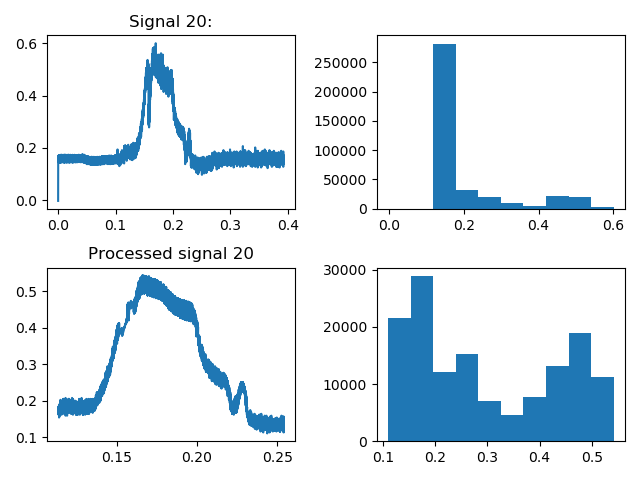
\includegraphics{threshold = 0.97 Num = 10 ShotNo= 38515 Signal= 20}}
		\caption{Параметр threshold = 0.97}
		\label{fig:threshold = 0.97}
	\end{figure}

	\begin{figure}[H]
		\center{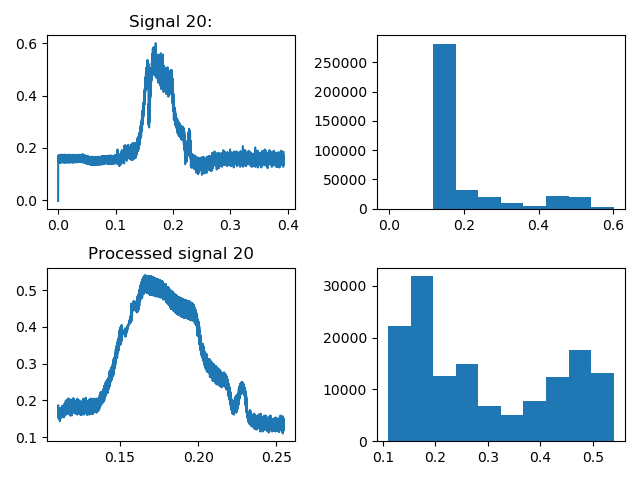
\includegraphics{threshold = 0.98 Num = 11 ShotNo= 38515 Signal= 20}}
		\caption{Параметр threshold = 0.98}
		\label{fig:threshold = 0.98}
	\end{figure}

	\begin{figure}[H]
		\center{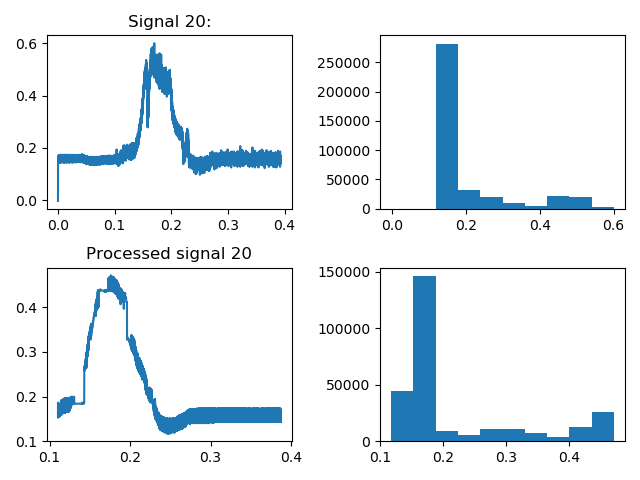
\includegraphics{threshold = 0.99 Num = 12 ShotNo= 38515 Signal= 20}}
		\caption{Параметр threshold = 0.99}
		\label{fig:threshold = 0.99}
	\end{figure}

\section{Обсуждение}
	Из рисунков выше можно сделать вывод о том, что при больших значениях параметра \underline{threshold} -  шум начинает считаться полезным сигналом например рисунок \ref{fig:threshold = 0.99}, при малых значениях - полезная часть считаеся шумом, например в рисунке \ref{fig:threshold = 0.01} пик гистограммы наименьший среди всех рисунков.Таким образом при зачениях параметра $0.21 - 0.81$ алгоритм можно считать устойчивым. 
	
	
	
	
	


\end{document}